
\section{Discussion}

\begin{figure*}[t]
  \centering
  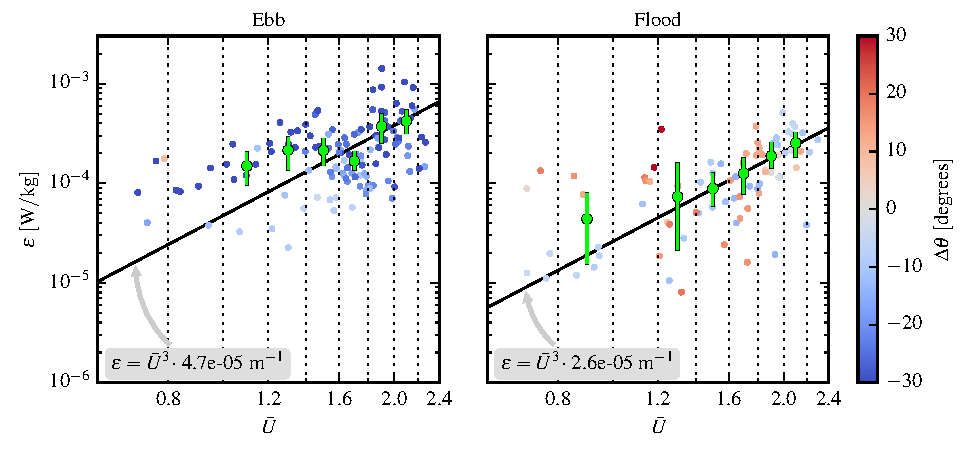
\includegraphics{EpsVU_TTM_02}
  \caption{$\epsilon$ versus $\bar{U}$ for the June 2014 TTM deployment during ebb (left), and flood (right). Small points are 5 minute averages, and their color indicates the angle of the mean horizontal velocity relative to the principal ebb or flood direction ($\Delta\theta=\theta-\theta_\circ$, where $\theta$ is the horizontal velocity direction, and $\theta_\circ$ is 310$^\circ$ and 130$^\circ$ true for ebb and flood, respectively).  Green dots are mean values within speed bins of 0.2 m s$^{-1}$ width that have at least 6 points (30 minutes of data); their vertical bars are 95\% bootstrap confidence intervals. The black line shows a $U^3$ slope, where the proportionality constant (grey box) is calculated by taking the log-space mean of $\epsilon/U^3$. }
  \label{fig:epsVu:ttm}
\end{figure*}

\begin{figure*}[t]
  \centering
  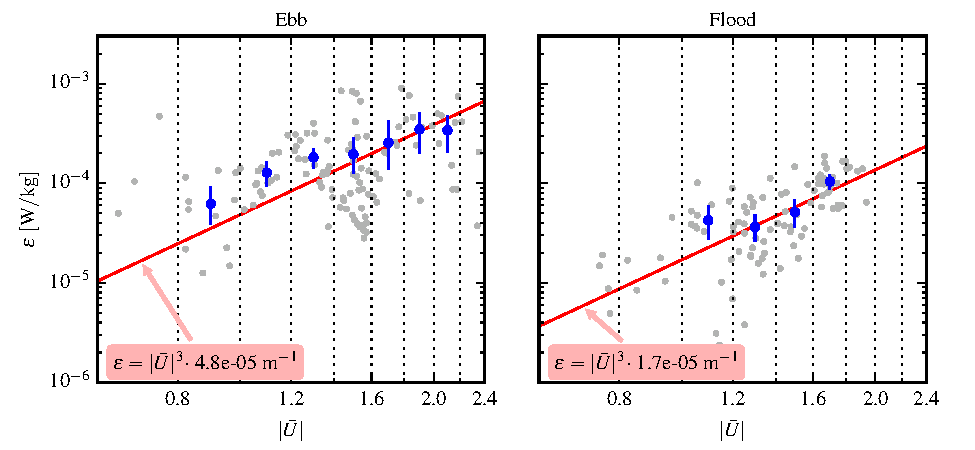
\includegraphics{EpsVU_SM_02}
  \caption{$\epsilon$ versus $\bar{U}$ for the May 2015 StableMoor deployment during ebb (left), and flood (right). The markers and annotations are identical to figure \ref{fig:epsVu:ttm}. }
  \label{fig:epsVu:sm}
\end{figure*}

This discussion needs to focus on turbulence measurements.

For many applications, such as estimating the turbulence dissipation rate, or turbulent kinetic energy, estimating the spectra is an intermediate step...
\begin{itemize}
\item $\uhead$ provides a justification, and a screening criteria(?), for removing portions of the signal.
\item Can estimate $\epsilon$, tke with fits that exclude contaminated portions of the spectra.
\item Can remove up to 10x signal motion
\item Discuss the time-domain method vs. spectral (cross-coherence) methods, and the need for phase information.
\item Should we estimate $\epsilon$ in this paper? If so, should this be in the Results section?
\end{itemize}



%%% Local Variables:
%%% mode: latex
%%% TeX-master: "Kilcher_etal_IMU-ADV"
%%% End:
